\section{Мотивация}

\begin{frame}{Что такое "проклятие размерности"?}
    $$
        S_{square}=1 \quad S_{circle}=\pi*(0.5)^2=\frac{\pi}{4}\approx0.79
    $$
    \begin{figure}
        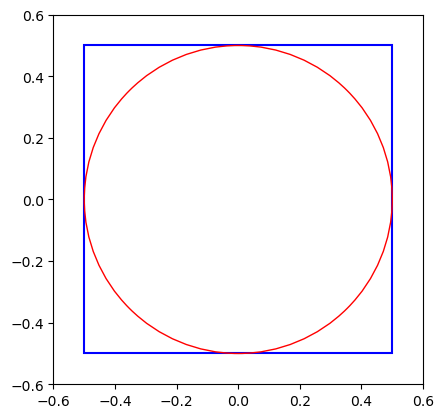
\includegraphics[width=0.55\textwidth]{../resources/motivation/inscribed_circle.png}
    \end{figure}
\end{frame}

\begin{frame}{Гиперсфера и гиперкуб}
    \begin{itemize}
        \item Объем гиперсферы стремится к нулю при росте размерности:
              \begin{equation*}
                  V_n = \frac{\pi^{n/2}}{\Gamma(\frac{n}{2}+1)}R^n
              \end{equation*}
        \item Диагональ гиперкуба увеличивается как \(\sqrt{n}\).
    \end{itemize}
    \begin{figure}
        \centering
        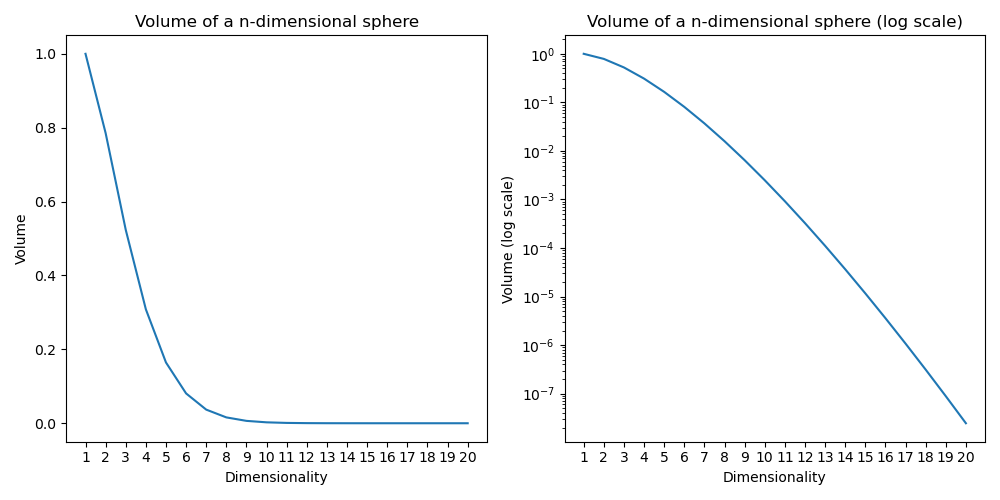
\includegraphics[width=0.7\textwidth]{../resources/motivation/sphere_volume.png}
    \end{figure}
\end{frame}
